%%%%%%%%%%%%%%%%%%%%%%%%%% author.tex %%%%%%%%%%%%%%%%%%%%%%%%%
%
% sample root file for your contribution to an IFIP volume
% published at Springer
%
% Use this file as a template for your own input.
%
%%%%%%%%%%%%%%%%%%%%%%%% Springer-Verlag %%%%%%%%%%%%%%%%%%%%%%%%%%


% RECOMMENDED %%%%%%%%%%%%%%%%%%%%%%%%%%%%%%%%%%%%%%%%%%%%%%%%%%%
\documentclass[ifip]{svmult}

% choose options for [] as required from the list
% in the Reference Guide, Sect. 2.2
\usepackage{url}
\usepackage{epsfig} 
\usepackage{makeidx}         % allows index generation
\usepackage{graphicx}        % standard LaTeX graphics tool
                             % when including figure files
\usepackage{multicol}        % used for the two-column index
\usepackage[bottom]{footmisc}% places footnotes at page bottom
\usepackage{float}           % H para posicionar figuras
\usepackage{booktabs}
% etc.
% see the list of further useful packages
% in the Reference Guide, Sects. 2.3, 3.1-3.3

\makeindex             % used for the subject index
                       % please use the style sprmidx.sty with
                       % your makeindex program


%%%%%%%%%%%%%%%%%%%%%%%%%%%%%%%%%%%%%%%%%%%%%%%%%%%%%%%%%%%%%%%%%%%%%

\begin{document}

\title*{Contribution Title}
% Use \titlerunning{Short Title} for an abbreviated version of
% your contribution title if the original one is too long
\author{Gema Rodriguez\inst{1}}
%\and Name of Author\inst{2}}
% Use \authorrunning{Short Title} for an abbreviated version of
% your contribution title if the original one is too long
 \institute{}
%\texttt{name@email.address}
%\and Name and Address of your Institute \texttt{name@email.address}}
%
% Use the package "url.sty" to avoid
% problems with special characters
% used in your e-mail or web address
%
\maketitle
\section{Introduction} 
\label{sec:1}

Many efforts on how and why bugs are introduced in the software source code are underway in the software engineering research community. Software source code is affected by many changes, many of them due to failure of the software because of emergent bugs. 

While a software system is being developed, software engineers use version repository to produce and manage their code. Developers and tester reported issues, which are stored in other repository known as issue-tracking system, when a wrong behavior or bugs are found in the systems.

Issue-tracking systems help solving these bugs, but their problem is the difficulty of distinguish the bug reports from other are not. These systems provide an interface to manage reports of maintenance activities. The developers report issues describing bug reports, features or optimizations. During the bug-seeding process is difficult distinguish bug reports from other issues due to the misclasification, a study describes that two of five issues was misclassified \cite{Herzig}. The misclassified causes bias predecting bugs whether non bug reports are taken into account.

To classify issues as bug reports or non bug reports we could use automatic classification system as is described in\cite{Antoniol}, but the vocabulary used in the issues could change as well as the policy depending on the project. Consequently, data validation is recomended in the studies\cite{Herzig}. 

Recording links between bug reports in a issue-tracking system and the corresponding fix-commit is a hard work, causing a lost time looking in issue-tracking systems and version repositories.

Traditionally, the methods used in link recovery \cite{Zimmermann, Thomas} are based on text patterns or the mining of key phrases. Unfortunately, this methods include several false negatives causing bias in data \cite{Bird, NguyenTH}. Therefore other methods could to be developed such as Mlink approach that links bug report with fixes using feauters in the changed source files corresponding to commit logs in addition to the traditional textual features \cite{Nguyen}. But all of them suppose that the issues are bug report. Hence, we propose a tool to display the data necessary to the developers/testers, who could decide whether the issue is a bug report or not. The developers know better than other the system,therefore the tool help their to choose only bug reports to be analyze in bug-seeding process removing any bias induced by non bug reports.
	

\section{The tool} 
\label{sec:2}
The tool works in the browser, displaying the main characteristics to distingush bug report from others in OpenStack project, the developers will be responsibles to classify the tickets as bug report or not, could explain his decisions in each ticket. 

OpenStack was particularly of interest because of its highest scope and heterogeneous nature with hundreds of developers contributing, futhermore due to its short life, only 5 years, all history is saved and available in a version control system. The issues are called tickets in OpenStack and availables in the Launchpad, a web interface of ticket tracking system, classifying them as bug report or not.

\subsection{Architecture}
This project works with Launchpad as issue-tracking system and Gerrit as code review system. The image \ref{fig:1} presents the architecture used in the tool, which has been developed with JavaScript, Node, JQuery and HTML5 technologies. The server side works making queries to the API of Gerrit an Launchpad, and the client side is where the user can see the information displayed. The client side interacts with the server through events. Both sides share the information requiered using JSON files. Futhermore, to integrate some funtionatities from github, we use a third-party application between github and the browser.

\label{sec:2.1}
\begin{figure}
\centering
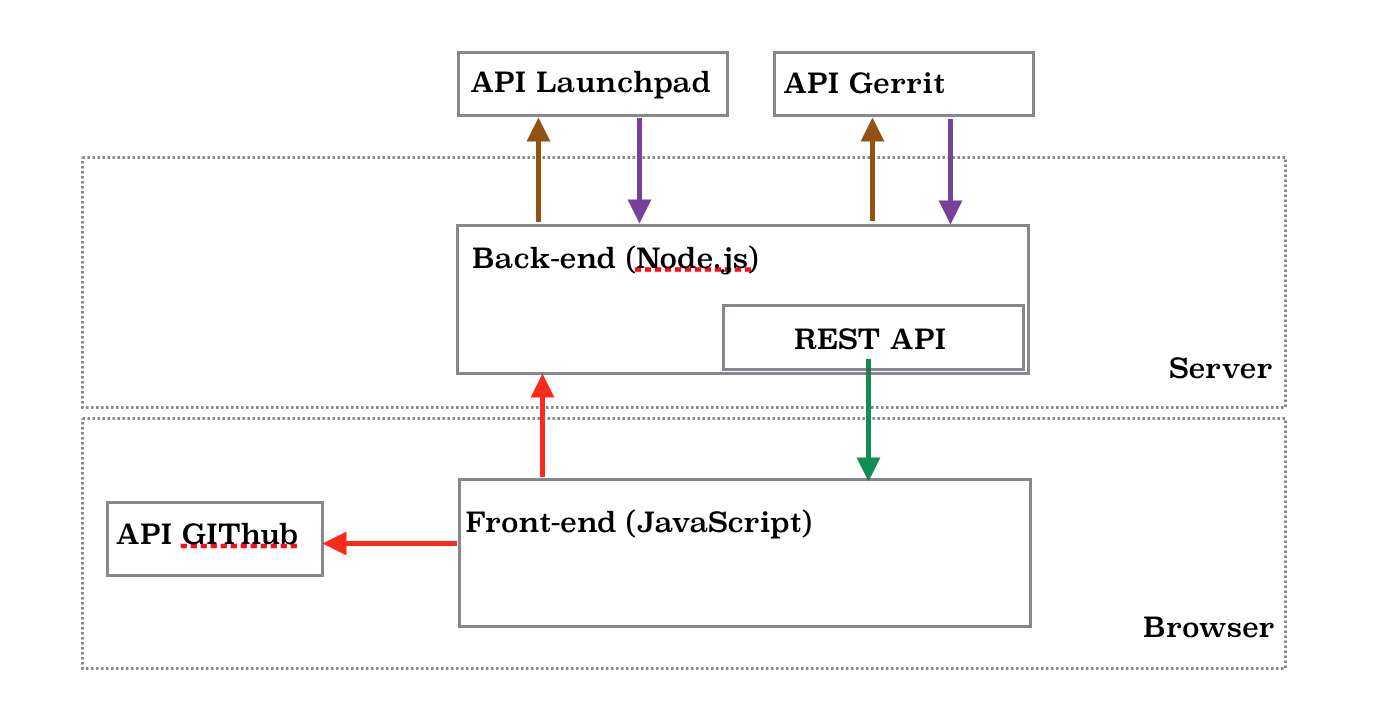
\includegraphics[height=4cm]{Arquitectura.png}
\caption{Architecture}
\label{fig:1}       % Give a unique label
\end{figure}

\subsection{Main Features}
\label{sec:2.2}
The tool shows the id of the tickets, which are extracted randomly from each issue-tracking repository of OpenStack, and displays the information necessary to decide whether the issue is a bug report or not. We focused in display the main parameters that help in the classification, such as the title of the report and the description as well as the description of the fix commit. 

The left side in the image \ref{fig:2}, shows the information related with the ticket in Launchpad and its correspondent fix-commit in Gerrit. Some information displayed link with the original pages in Launchpad and Gerrit, thereby the  developers have at their disposal extra information such as the comments that other developers have done. Could tracking the history since the ticket opens until the commit fixed the ticket.

The right side is guided to user's opinion, after reading all the information displayed, they have to classify the ticket as \textit{Bug report} or \textit{Not Bug report}. Due to unsophisticated description used in the ticket, the developers could doubt in the classification, for this reason we add an extra option in the classification, \textit{Undecided}. Futhermore, the developers have a textarea to write their opinion about their classification in each ticket, as well as other textareas to write the keywords found in the title and the description which can help us building an automatic classification system in the future.

The tool allow carry out a double bind analisys, due to the data is saved in github user's account. In order that, the user can only see and modify their own data saved. Github is a control version system in which we have access to the whole information of each commit submitted by the developer. Thus, saving the data in Github, we could measure the time that each developer spend in the analisys, which tickets were more difficult to anaylize and other statistics that can help us undertanding the current problem of issues misclassification.

We continue developing the tool but an initial version is available \footnote{\url{bugtracking.libresoft.es}}, as well as a demonstration video\footnote{\url{https://www.youtube.com/watch?v=q0-TIvL4mqc&feature=youtu.be}}. It presents a licence type GPL 0 (General Public License) and you can find the code in my github's account\footnote{\url{https://github.com/Gemarodri/BugTracking}}. Anyone can use it regardless of have github account or not. But, they only can save and modify their data, in addition, one of the requirements to save and modify data is create a new repository with the same name that the repository of OpenStack you want to analyze. 

\begin{figure}
\centering
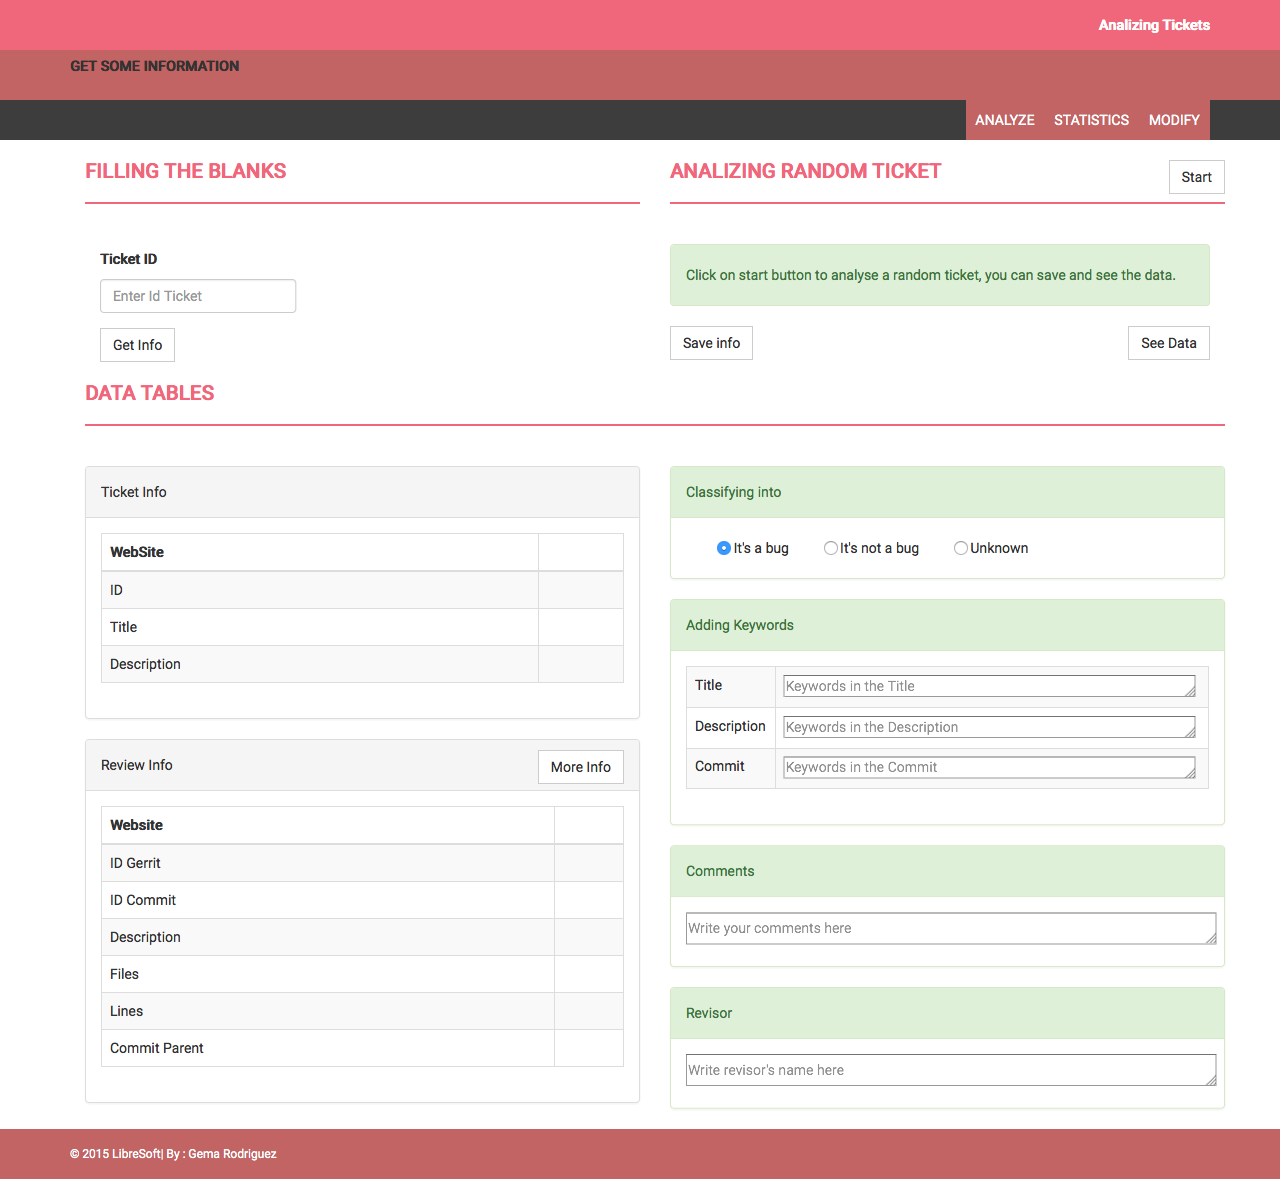
\includegraphics[height=10cm]{index.png}
\caption{Screenshot of Index}
\label{fig:2}       % Give a unique label
\end{figure}
\section{Validation Study} 
\label{sec:3}

We use the tool to analyze randomly 500 tickets, reported in the last year, from the four principal repositories in OpenStack. This tickets could be tagged as either "Fix Commited" or "Fix Released", to be able to localizate the patch implemented into de source code in the version repository. They are generally tracked in Launchpad \texttt{Nova},\texttt{Cinder},\texttt{Horizon} and \texttt{Neutron}\footnote{\url{https://bugs.launchpad.net/NameOfRepository}}

The parameters analyzed for each ticket were the title and the description of the report and the description of the fix commit. Also, the code changes if neither the descriptions and the comments clarified the underlying tiket. Each ticket was then categorized into one of three following groups.
\begin{enumerate}
  \item The ticket describes a bug report.
  \item The ticket describes a feature, an optimitazion code, changes in test files or other not bug reports.
  \item The ticket presents a vague description and cannot be classified without doubts. 
\end{enumerate}

Henceforth, we will refer to Group 1 as \textit{Bug Report}, Gruop 2 as \textit{not Bug Report} and Group 3 as \textit{Undecided}.

In the analisys were involved three different developers who used a double bind review process, obtaining that each tickets was analyzed by two developers. Each developer analyzed 167 tickets plus the half tickets of his teammates. %Only at the end, they disscused the classification conflicts to reach an agreement.
 
\section{Results} 
\label{sec:4}
We have manually analyzed 500 tickets with support of the present tool. The table ~\ref{tab:1} show the statistics of each developer after analysed 334 tickets. 

\begin{table}[htb]
\begin{center} {\footnotesize
\caption{ Classification statistics of each developer}
\label{tab:1}
\begin{tabular}{llll}
\toprule[0.3mm]%{\smallskip}
  & Bug Report\kern 1pc & Not Bug Report\kern 1pc & Undecided \\\hline
Developer 1 \kern 1pc & 53.89\% & 34.13\% & 11.98\% \\
Developer 2 \kern 1pc & --\% & --\% & --\% \\
Developer 3 \kern 1pc & --\% & --\% & --\% \\
\bottomrule[0.3mm]
\end{tabular} }
\end{center}
\end{table}

(should we corroborate that the statistics are similar with the previous study where only 100 tickets were analyse?\\
results with 100 tickets: (63\%) have been considered as Bug Report, (21\%) as Not Bug Report, and (16\%) as Undecided) 
)
% Developer 1: 334 tickets
% H--Ne--C--No
% 64+50+31+35 --> 180 -->(53.89%)
% 45+26+24+19 --> 114 -->(34.13\%)
% 16+7+8+9 --> 40 --> (11.98\%)

\section{Discussion}
\label{sec:5}
How to procede if there are discordances beetween the developers:

- Should the developers disscuss after their analisys to reach a better classification?
- Does the bug report only the same ticket classified as Bug report for all the developers?

\subsection{Future Work}
\label{sec:5.1}

We would like know what grade of responsability, none or totally, practice the previous commit in the seeding of a bug in OpenStack, considering that currently exists an implicit assumption: the line that contains the error was caused by the inmediately previous commit\cite{Sliwerski}. The accuracy in our results depends on the quality of the data, thus we should focus only on bug reports discarding the other issues.

- Implement this part in the tool, displaying the code after and before the bug fixed and after and before the bug-introduction to determinate if the previous commit is responsible or not.

\section{Knowleadges}
\label{sec:6}

%%%%%%%%%%%%%%%%%%%%%%%% referenc.tex %%%%%%%%%%%%%%%%%%%%%%%%%%%%%%
% sample references
% "computer science"
%
% Use this file as a template for your own input.
%
%%%%%%%%%%%%%%%%%%%%%%%% Springer-Verlag %%%%%%%%%%%%%%%%%%%%%%%%%%

%
% BibTeX users please use
% \bibliographystyle{}
% \bibliography{}
%
% Non-BibTeX users please use
\begin{thebibliography}{99.}
%
% and use \bibitem to create references.
%
% Use the following syntax and markup for your references
%
% Monographs
%\bibitem{monograph} Kajan E (2002)
%Information technology encyclopedia and acronyms. Springer, Berlin
%Heidelberg New York

% Contributed Works
%\bibitem{contribution} Broy M (2002) Software engineering -- From
%auxiliary to key technologies. In: Broy M, Denert E (eds)
%Software Pioneers. Springer, Berlin Heidelberg New York
\bibitem{Antoniol}Antoniol, G., Ayari, K., Di Penta, M., Khomh, F., \& Gu\'eh\'eneuc, Y. G. (2008, October). Is it a bug or an enhancement?: a text-based approach to classify change requests. In Proceedings of the 2008 conference of the center for advanced studies on collaborative research: meeting of minds (p. 23). ACM.
\bibitem{Herzig}Herzig, K., Just, S., \& Zeller, A. (2013, May). It's not a bug, it's a feature: how misclassification impacts bug prediction. In Proceedings of the 2013 International Conference on Software Engineering (pp. 392-401). IEEE Press.
\bibitem{Sliwerski}J. Śliwerski, J., Zimmermann, T., \& Zeller, A. (2005, May). When do changes induce fixes?. In ACM sigsoft software engineering notes (Vol. 30, No. 4, pp. 1-5). ACM.
\bibitem {Nguyen}Nguyen, A. T., Nguyen, T. T., Nguyen, H. A., \& Nguyen, T. N. (2012, November). Multi-layered approach for recovering links between bug reports and fixes. In Proceedings of the ACM SIGSOFT 20th International Symposium on the Foundations of Software Engineering (p. 63). ACM.
\bibitem {Zimmermann}Zimmermann, T., Premraj, R., \& Zeller, A. (2007, May). Predicting defects for eclipse. In Predictor Models in Software Engineering, 2007. PROMISE'07: ICSE Workshops 2007. International Workshop on (pp. 9-9). IEEE.
\bibitem{Thomas}Zimmermann, T., \& Weißgerber, P. (2004, May). Preprocessing CVS data for fine-grained analysis. In Proceedings of the First International Workshop on Mining Software Repositories (pp. 2-6). sn.
\bibitem{Bird}Bird, C., Bachmann, A., Aune, E., Duffy, J., Bernstein, A., Filkov, V., \& Devanbu, P. (2009, August). Fair and balanced?: bias in bug-fix datasets. In Proceedings of the the 7th joint meeting of the European software engineering conference and the ACM SIGSOFT symposium on The foundations of software engineering (pp. 121-130). ACM.
\bibitem{NguyenTH}Nguyen, T. H., Adams, B., \& Hassan, A. E. (2010, October). A case study of bias in bug-fix datasets. In Reverse Engineering (WCRE), 2010 17th Working Conference on (pp. 259-268). IEEE.
% Journal
%\bibitem{journal} Che M, Grellmann W, Seidler S (1997)
%Appl Polym Sci 64:1079--1090




% Theses
%\bibitem{thesis} Ross DW (1977) Lysosomes and storage diseases. MA
%Thesis, Columbia University, New York

\end{thebibliography}

%%%%%%%%%%%%%%%%%%%%%%%%%%%%%%%%%%%%%%%%%%%%%%%%%%%%%%%%%%%%%%%%%%%%%%

%%%%%%%%%%%%%%%%%%%%%%%%%%%%%%%%%%%%%%%%%%%%%%%%%%%%%%%%%%%%%%%%%%%%%%

%\printindex
\end{document}





